\subsubsection{Как строятся каскады на ОИ,ОЗ,ОС?}

Преимущество УПТ - они управляются входоным напряжением: в транзисторах с объемным каналом затвор отделен от канала обедненным слоем p-n перехода, а в транзисторах с приповерхностным слоем (МОП) - слоем диэлектрика.
В усилительном каскаде все транзисторы работают на пологом участке ВАХ: максимальное значение крутизны и коэффициента усиления (\~S):
$$
S=b*[U_{}-U_{porogovoe}]
$$
В усилителе на УПТ стоко-затворная ВАХ - квадратичная функция, следовательно при большом сигнале будут явные нелинейные искажения
\begin{center}
\begin{figure}[h!]
\center{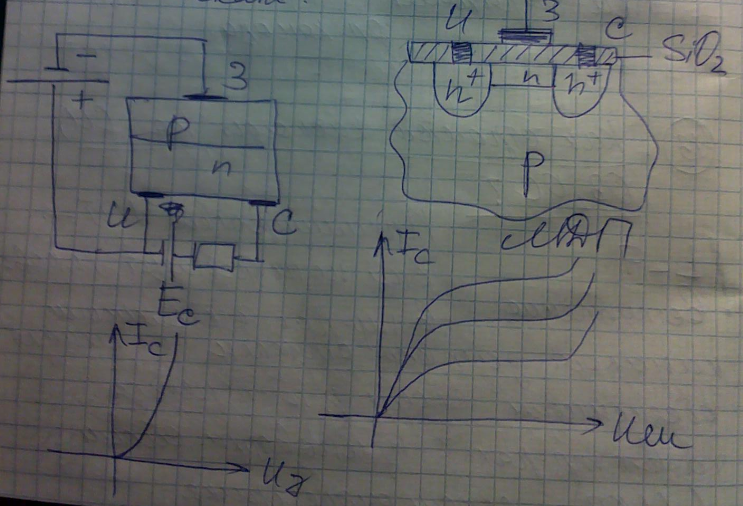
\includegraphics[scale=0.7]{p3_13.png}}
\end{figure}
\end{center}
(далее про все 3 каскада)
